\documentclass[hyperref={pdfpagelabels=true}]{beamer}

\usepackage{lmodern}
\usepackage{hyperref}
\usepackage{caption}
 
\title{Predictive Analysis of Road Incidences}   
\subtitle{Exploratory Lines}
\author{BDigital} 
\date{\today} 
\titlegraphic{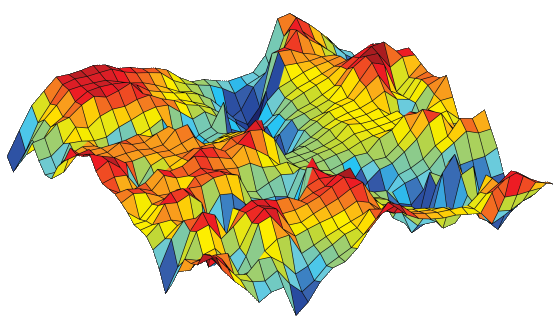
\includegraphics[width=.45\textwidth,height=.35\textheight]{som.png}}
 
\usepackage{beamerthemeshadow}
%\usepackage{beamerthemesplit}
\usepackage{listings}

\newcommand{\soooo}{H$_2$SO$_4$}

%fdl stuff
\usepackage{hyperref}
\hypersetup{colorlinks, 
           citecolor=black,
           filecolor=black,
           linkcolor=black,
           urlcolor=black,
           bookmarksopen=true,
           pdftex}

\hfuzz = .6pt % avoid black boxes

\begin{document}

\captionsetup{font=scriptsize,labelfont=scriptsize}

\setbeamertemplate{footline}[page number]
\setbeamertemplate{navigation symbols}{}
\begin{frame}
\titlepage
\end{frame} 
 
\begin{frame}
\frametitle{Introduction}
\begin{overprint}
\begin{itemize}
\item Despite significant improvements in vehicle technology and road engineering over the last 40 years, on a world-wide scale 
road accidents are still one of the main accidental causes of death and injury (WHO, 2004).\\
%The assessment of the occurrence of road accidents and the management of infrastructure to deal with this risk are therefore research areas of considerable interest. 
\item In a study regarding the relation between extreme weather events (e.g.: flash floods) and road accidents it was found that motorists account for 84 \% of the totality of the
victims~\cite{calabria}.
%Identification of factors that affect the occurrence of road accidents has attracted the attention of many researchers in the field of traffic
%safety.\\%Recognizing such elements may help not only to reduce the number of deaths in traffic crashes, but also the number of accidents with severe injuries [cite].\\ 
\item The assessment of the occurrence of road accidents has therefore attracted the attention of many researchers.
\end{itemize}
\end{overprint}
\end{frame}
\begin{frame}
\frametitle{Introduction (cont.)}
\begin{figure}
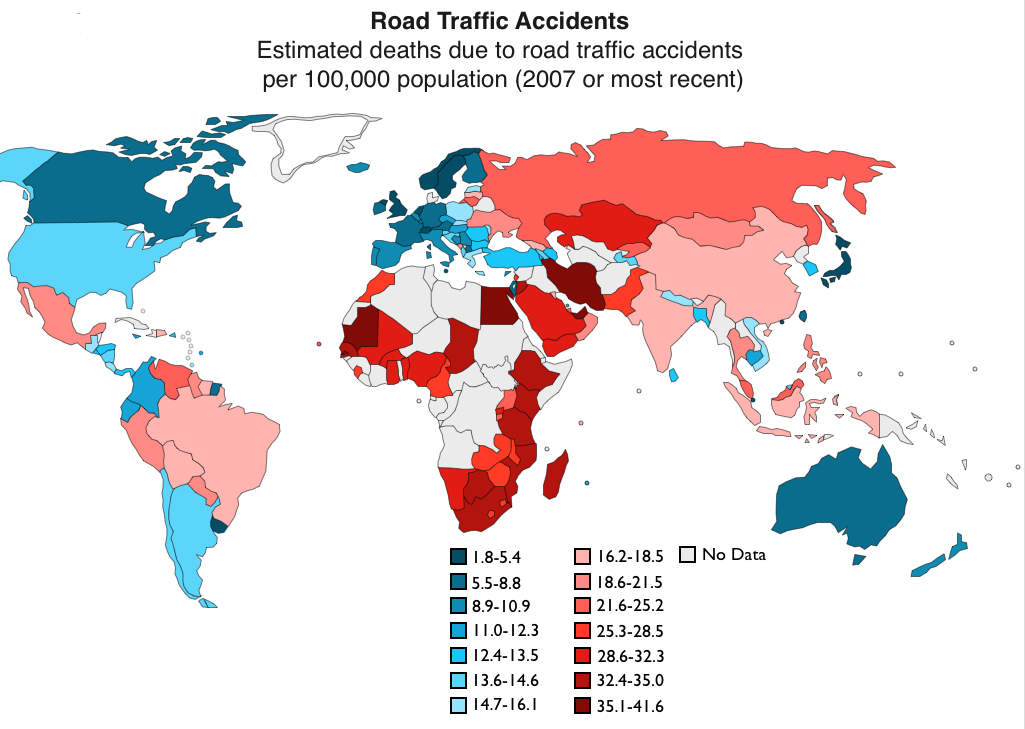
\includegraphics[scale=0.25]{world_accidents.png}
\end{figure}
\tiny{source: {\url http://www.geocurrents.info}}
\end{frame}

\begin{frame}
\frametitle{Research Question}
\textbf{ What do we want to predict?}\\
Ocurrence (0,1) and location (x,y) of incidents, as a function (pairwise or multivariant) of other variables;
\small{
\begin{itemize}
\item time of the day;
\item weekday;
\item traffic density;
\item weather (rainfall, snowfall, visibility, winds, etc);
\item traffic control devices (e.g.: traffic lights, stop signal, etc);
\item roadway geometries (e.g.: steepness, intersection, degree of curvature, etc) 
%\footnote{\tiny{Factors reflecting basic road geometry and traffic volumes have been demonstrated to have a 95\% significance level[cite]}}
;
\item roadway conditions (road surface, obstacles);
%\item driver behavior
\item vehicle type;
%\item human conditions (characteristics of the driver, fatigue, alcohol);
%\item involvement of pedestrians;
\end{itemize}
}
Some of these variables are continuous in space and most of them change over time.\\
\end{frame}

\begin{frame}
\frametitle{Modelling Approaches: Classical Statistics}
\begin{itemize}
\item<1-> The most common approach applied in early works is to model the interaction between each dependent variable and incidence frequencies by means of conventional (multiple) linear regression models~\cite{bayesian}; these \textbf{do not take in account covariance between response variables}. 
\item<2-> Most of these models use a Normal or Poisson distribution that is not well-suited to the scarce nature of incidence data. Accident data is often characterized by small observed mean values and a large number of zero counts leading to the well discussed phenomenon of \textbf{over-dispersion}: the presence of greater variability (statistical dispersion) in a data set than would be expected based on a given simple statistical model.
\item<3-> None of these models addresses explicitly the question of \textbf{spatial autocorrelation}: the value of samples taken close to each other are more likely to have similar magnitude than by chance alone.
\end{itemize}
\end{frame}

\begin{frame}
\frametitle{Modelling Approaches: Data Mining}
Statistical models are particularly likely to be preferable when fairly simple models are adequate and the important variables can
be identified before modeling. \textbf{This is not the case of the large and complex data set of road incidences}.\\
%\footnote{\tiny{It should be noted that more complex models such as Negative Binomial (NB) and Poisson-lognormal are able to overcome these limitations}} [cite]
%Poisson NB: they have their own assumptions and pre-defined underrlying relationship between dependent and independent variables
%. If these assumptions are violated, the model could lead to erroneous estimation of accident likelihood.
\vspace{5mm}
\textbf{Data mining} can be defined as the \textit{nontrivial process of identifying valid, novel, potentially useful, and ultimately understandable patterns in large amounts of data} ~\cite{sets}.
\small{
\begin{itemize}
%\item It can be viewed as a computer automated exploratory data analysis of (usually) large complex data sets [cite].
\item<1-> Scale differences: data sets can be much larger than in statistics.
\item<2-> Conceptual differences: compared with statistics, data mining pays less attention to the large-scale asymptotic properties of its inferences and more to the general philosophy of \textit{learning}. For this fact, data mining has been criticized for being a "black box"~\cite{zeng}.
\item<3-> Dataset collection differences: it is generally a form of secondary data analysis, as very likely the datasets have been collected for other purpose than the one of answering the research question.
\end{itemize}
}
\end{frame}

\begin{frame}
\frametitle{Data Mining}
There are two major groups of tasks in Data Mining~\cite{sets}:
\begin{itemize}
\item Description: affinity group and clustering;
\item Prediction: classification and estimation;
\end{itemize}
\begin{figure}
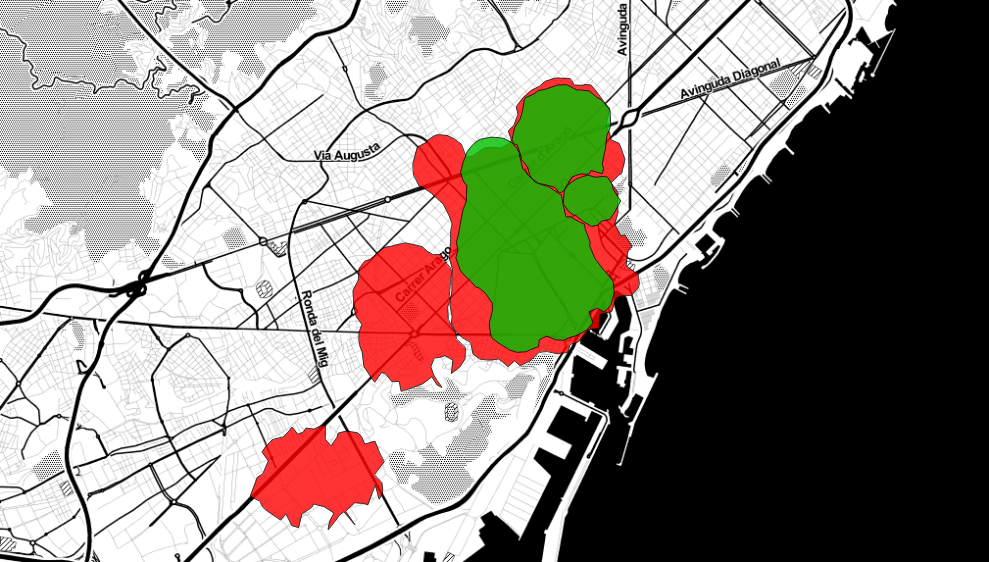
\includegraphics[scale=0.35]{mwc_nonmwc_1000_0125.png}
\end{figure}
\tiny{DBSCAN clusters of tweets during MWC vs a \textit{normal} day}
\end{frame}

\begin{frame}
\frametitle{Modelling Techniques}
Often Data Mining Techniques are combined together, or with traditional statistical methods, to yield better results:
\begin{itemize}
\item \textbf{Multivariate regression analysis + Bayesian Probabilistic Networks (BPN)}~\cite{bayesian};
\item Random Forest + Multivariate Adaptive Regression Splies (MARS)~\cite{mars};
\item Classification and Regression Trees (CART)~\cite{cart};
\item Genetic Mining Rule + Logit Model~\cite{gmr};
\item \textbf{Frequent Item Sets}~\cite{sets};
\item Support Vector Machines (SVM); 
\item \textbf{Self Organizing Maps (SOM)};
%both present accuracies above 90%[cite]; SOM are only slighlty worst than SVM, which is unsuprising since they are trained in an unsuperviced fashion; they provide usefull graphic representations.
\end{itemize}
\end{frame}

\begin{frame}
\frametitle{Bayesian Approach}
In this case study~\cite{bayesian} it is used a mixed-model to predict the ocurrence of road accidents:
\begin{itemize}
\item<2-> Multivariate Poisson-lognormal regression analysis, which facilitates taking into account the covariance structure of the model response variables as well as
over-dispersion effects.
\item<3->  Bayesian Probabilistic Networks (BPN) that take into account aleatory and epistemic uncertainties as well as possibly non-linear dependencies between the risk indicating variables and the response variables.
\end{itemize}
The BPN is based on the regression model, but its parameters are updated by learning algorithms; the update \textit{only replaces the response variables that have been observed in conjunction with the accident}. This approach allows to cope with different degrees of completness of the dataset.\\
The methodology is illustrated using data of the Austrian rural motorway network (+/- 80 000 vehicles/day) and the quality of the prediction was found to be 73\%.
\end{frame}

\begin{frame}
\frametitle{Association Algorithm}
In this case study~\cite{sets} an association algorithm is used to obtain a descriptive analysis of accident high risk areas. This algorithm \textbf{identifies the accident circumstances that frequently occur together}. We are able to target the highest frequencies through a \textit{minimum support value}.\\
This algorithm was applied to road accident data in Belgian (1997-1999). 
%The dataset is long enough to limit random fluctuations in the accident counts and short enough to limit changes in road and traffic conditions.
Some factors that were frequently linked to accidents:
\begin{itemize}
\item "Left" turns;
\item Uneven views when approaching an intersection;
\item Rainy conditions;
\item Involvement of young pedestrians;
\end{itemize}
Some of these risk factors could be reduced with signing or roundabouts in these zones;
\end{frame}

\begin{frame}
\frametitle{What About Space?}
 \small{\center{\textit{Everything is related to everything else, but closer things are more closely related.}}\\ \hfill Tobler, 1970}
\begin{figure}
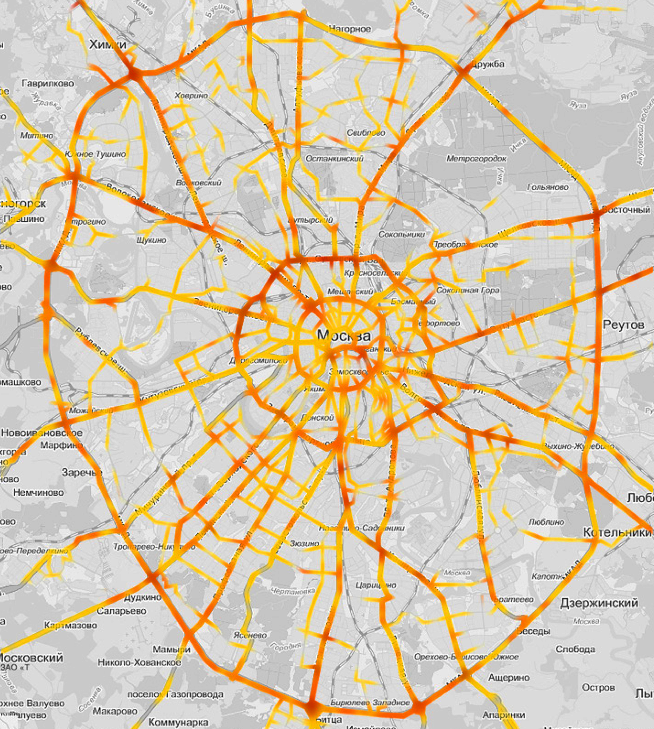
\includegraphics[scale=0.2]{accidentmap.png}
\caption{\tiny{Heat map of road accidents in Moscow; source: {\url http://mapsforhumans.com/2011/07/road-accidents-heat-map-of-moscow/}}}
\end{figure}
\end{frame}

\begin{frame}
\frametitle{What About Space? (cont.)}
Road incidences happen in time and \textbf{space}. The contact with the spatial dimension of the phenomena starts with the input dataset.\\
%Often accident data comes in very small units (e.g.: 100 m). Sometimes a spatial aggregation can be recommended, for getting rid of location error, and
%also to increase the magnitude of the results. We have to be very carefull on how-to do this generalisation.\\
The most frequent approach to represent the road structure is to use networks. Networks represent lanes as \textit{links} and intersections as \textit{nodes}.
\begin{figure}
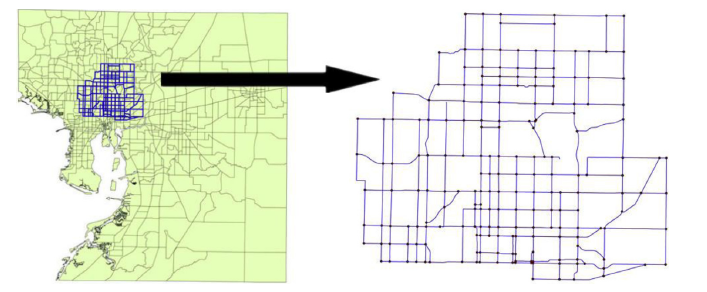
\includegraphics[scale=0.40]{road_network.png}
\caption{\tiny{Road network in  Hillsborough~\cite{zeng}}}
\end{figure}
For longer roads, it may be actually useful to split them into \textbf{homogeneous sections}. %There are also \textit{gridifications} of these networks [cite].
\end{frame}

\begin{frame}
\frametitle{What About Space? (cont.)}
But the space dimension does not cease in the representation of the input variables (implicit). Space \textbf{relationships should also be explicitly stated in the model}.
\begin{itemize}
\item Spatial Auto correlation (as opposed to spatial independence) is an arrangement of the accidents where the locations are related to each other.
\item Numerous studies have shown that accounting for spatial correlation among the analyzed observations is a big step toward a better safety assessment~\cite{zeng}.
\item This is actually a \textit{weakness} of many models; on the Baysean Network model~\cite{bayesian}, although acknowledged, spatial correlations were not considered in the development of the risk model; on conditionally autoregressive models (CAR) spatial effects are introduced as random.
\end{itemize}
Geographical Information Systems (GIS) can be a valuable tool for representing/integrating the different variables on a geographical space.
\end{frame}

\begin{frame}
\frametitle{Considering Space: A Simple Example}
Study of how circumstances affect people in episodes of bad weather~\cite{calabria}.Data from newspappers was collected for a period of 10 yrs, in the region of Calabria.
\begin{figure}
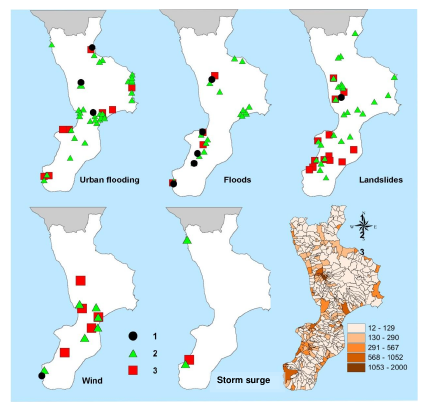
\includegraphics[scale=0.55]{damage_agent.png}
\caption{\tiny{Localisation of damage to people sorted according to the type of damaging agent. (1) Victims, (2) injured, and (3) involved people~\cite{calabria}}}
\end{figure}
\end{frame}

\begin{frame}
\frametitle{Considering Space: A Simple Example (cont)}
\begin{columns}
  \begin{column}{0.5\textwidth}
    \begin{figure}
    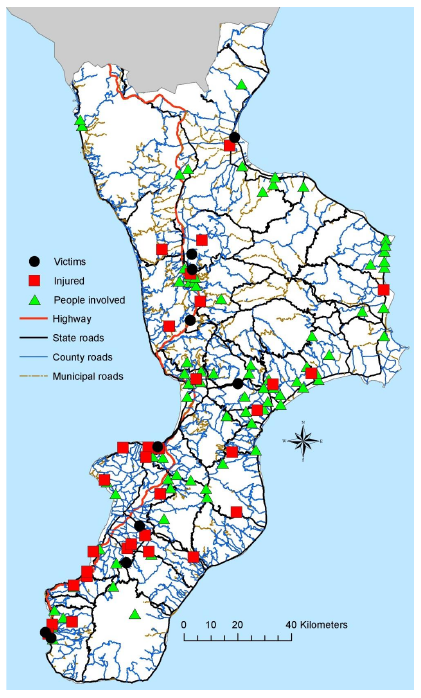
\includegraphics[scale=0.4]{damage2.png}
    \caption{\tiny{ Localisation of damage to people along the Calabria road network~\cite{calabria}}}    
    \end{figure}
  \end{column}
  \begin{column}{0.5\textwidth}  
  \small{
  \begin{itemize}
  \item Urban flooding and flash floods were found to be the most damaging events;
  \item Drivers accounted for 84\% of the victims during these episodes.
  \item The mapping of damaging effects pointed out the regional sectors for which the high frequency of damaging events suggests planning further in-depth examinations; 
  \item The identification of these crictical points can support local regulator interventions, that might change damage incidences in the future.
  \end{itemize} }
  \end{column}
\end{columns}
\end{frame}

\begin{frame}
\frametitle{Considering Space: A more complex example}
The Self Organizing Map (SOM) is an artificial neural network based on an unsupervised learning process that performs a gradual and nonlinear mapping of high dimensional input data onto an ordered and structured array of nodes, generally of lower dimension~\cite{gorricha}.
\begin{itemize}
\item <1-> The SOM compresses information and reduces dimensionality;
\item <2-> It transforms nonlinear statistical relationships in geometric relationships;
\item <3-> It is a visualization method for multidimensional data;%visual data mining
\item <4-> Unlike other NN models, it \textbf{preserves topological relationships} units that are close in the output space, are also next to each other in the data space.%neighborhood function
\item <5-> Unlike other models (e.g.: Support Vector Machines), as the training is unsupervised, it can prevent the analyst's arbitrary perspective.%undirected knowledge discovery
\end{itemize}
\end{frame}

\begin{frame}
\frametitle{Self Organizing Maps}
The process of creating SOMs undergoes two main stages~\cite{goat}:
\small{
\begin{itemize}
\item <2-> training: vector quantitization; the neurons \textit{adjust} their weights to the input vector;
\item <3-> mapping: vector projection; the network classifies a new input dataset;
\end{itemize}
}
\begin{figure}
\includegraphics[scale=0.35]{colors.png}
\caption{\tiny{source: \url{http://www.mql5.com/en/articles/283}}}
\end{figure}
\end{frame}

\begin{frame}
\frametitle{Self Organizing Maps (cont.)}
\small{Apart from the predictive capacity, the algorithm also works as a multidimensional clustering algorithm and a valuable visualization tool (U-Matrix and component planes).}
%u-matrix depicts the units distance in grayscale
\begin{figure}
\includegraphics[scale=0.25]{som2.png}
\caption{\tiny{source: \url{https://upload.wikimedia.org/wikipedia/commons/7/70/Synapse_Self-Organizing_Map.png}}}
\end{figure}
\end{frame}

\begin{frame}
\frametitle{Self Organizing Maps (cont.)}
When applied to geo-referenced data, this technique may allow the
explanation of complex structures and phenomena in a spatial perspective~\cite{gorricha}.\\
\vspace{5mm}
Going back to geographical space:
%we transformed the data space in output space, but we can go back to the data space
\begin{columns}
  \begin{column}{5cm}
    \begin{figure}
    \includegraphics[scale=0.4]{poverty1.jpg}
    \end{figure}
  \end{column}
  \begin{column}{5cm}
    \begin{figure}
    \includegraphics[scale=0.33]{poverty2.jpg}
    \end{figure}
  \end{column}
\end{columns}
\tiny{source: \url{http://www.ai-junkie.com/ann/som/som5.html}}\\
\end{frame}

\begin{frame}
\frametitle{Self Organizing Maps (cont.)}
SOM's have been used for estimating:
\begin{itemize}
\item the risk for cancer patients (demonstrated accuracy in classification)~\cite{cancer};
\item underlying physical parameters from near infrared planetary spectra (83\%-100\% accuracy)~\cite{infrared};
\item the distance of an astronomic object based on its color (when compared to other techniques offer a competitive choice in terms of low-RMSE, and percentage of outliers)~\cite{redshift};
%root-mean-square error
\item productivity of goat and sheep farms, based on herd management practices (the results are coherent with the animal science criteria that are common for this problem)~\cite{goat};
%\item types of accident crashes (e.g.: drunk speeding, intersection, etc)[cite];
\end{itemize}
The approach has been showed to be an evidence-based predictive tool with high-knowledge-generation capabilities, very valuable to support decision-making ~\cite{cancer}.
\end{frame}

\begin{frame}
\frametitle{SOM's and Road Incidences}
\begin{itemize}
\item Real-world road incidences are characterized by complicated multi-dimensionality mutual relationships.
\item We want to propose a SOM to capture and extract the essence of these relationships by visualizing the results of incidence clustering.
\item Moreover, we want to be able to predict these clusters of incidences, for a new set of input variables.
\end{itemize}
SOMs have been used in a study to estimate the effectiveness of Crash Avoidance technologies~\cite{crash}. They identified and characterized clusters of accidents, based on the relationships between (normalized) variables.
\begin{itemize}
\item <2-> 1 year of data (2010);
\item <3-> 16,180 fatal passenger car drivers;
\item <4-> 48 variables;
\end{itemize}
\end{frame}

\begin{frame}
\frametitle{Discussion}
\begin{itemize}
\item What incidence dataset could we use? (e.g.: time and space dimensions, magnitude of incidence, type of incidence);
\item Incidences vs Accidents;
\item Would it be possible to have two datasets: one for training and one for validation?
\item What type of predictive dataset do we have (e.g.: road geometry, road characteristics, traffic density) ?
\item How accurate are these datasets (measuring errors, etc)?
\end{itemize}
\end{frame}

\begin{frame}
\frametitle{More: Targeting Specific Aspects of Incidences:}
These are examples of studies that focus on specific aspects of road incidences:
\begin{itemize}
\item Identify and describe secondary crashes~\cite{secondary};%developed analysis framework : identify and describe secondary crashes
\item Identify hots pots or "black zones", and model their behaviour~\cite{bayesian};
\item Model crashes at specific type of road entity (e.g.: unsignalised intersections)~\cite{mars};%mars model
\item Model accident severity (casualties or damages)~\cite{severity};%casualties or damages; classification that leads to prediction
\end{itemize}
\end{frame}

\begin{frame}
\frametitle{More: Other Relevant Studies:}
These are examples of other traffic-related studies, that do not focus on incidences:
\begin{itemize}
\item Predict traffic levels in unmeasured locations (Kriging)~\cite{kriging};
\item Evaluate the level of road traffic congestion (MCE, ANN)~\cite{congestion};%traffic jam. evaluated by measuring accuracy of outputs against human opinion.
\item Traffic simulation model (CA)~\cite{ca};%Large scale microscopic traffic simulation using CA is simpler to implement on computers, provides a sim- ple physical picture of the system and can be easily modified to deal with different aspects of traffic. However,
%\item Traffic Forecast System[cite];
\item Predict travel time~\cite{traveltime};%use data-mining techniques, K-means, NN, etc
\end{itemize}
\end{frame}

%\begin{frame}
%\frametitle{Visualization}
%3D viz: give some "eye candy" examples
%\end{frame}

\begin{frame}[allowframebreaks]
\frametitle{References}
\tiny{
 \begin{thebibliography}{ab}
  \bibitem{calabria} O. Petrucci and A. A. Pasqua {\em Damaging events along roads during bad weather periods: a case study in Calabria (Italy)}. Nat. Hazards Earth Syst. Sci., 12, 365-378, 2012. 
  \bibitem{bayesian} Markus Deublein and Matthias Schubert and Bryan T. Adey and Jochen Kohler and Michael H. Faber {\em Prediction of road accidents: A Bayesian hierarchical approach}. Accident Analysis \& Prevention 51, 274-291, 2013.
  \bibitem{sets} Karolien Geurts and Isabelle Thomas and Geert Wets {\em Understanding spatial concentrations of road accidents using frequent item sets}. Accident Analysis and Prevention 37, 787-799, 2005.
  \bibitem{zeng} Qiang Zeng and Helai Huang {\em Bayesian spatial joint modeling of traffic crashes on an urban road network}. Accident Analysis \& Prevention 67, 105-112, 2014.
  \bibitem{gmr} Yu-Chiun Chiou and Lawrence W. Lan and Wen-Pin Chen {\em A two-stage mining framework to explore key risk conditions on one-vehicle crash severity}. Accident Analysis \& Prevention 50, 405-415, 2013.
  \bibitem{cart} Li-Yen Chang and Wen-Chieh Chen {\em Data mining of tree-based models to analyze freeway accident frequency}. Journal of Safety Research 36, 365-375, 2005.
  \bibitem{mars} Mohamed Abdel-Aty and Kirolos Haleem {\em Analyzing angle crashes at unsignalized intersections using machine learning techniques}. Accident Analysis \& Prevention 43, 461-470, 2011.
  \bibitem{gorricha} Jorge Manuel Lourenco Gorricha {\em Visualization of Clusters in Geo-referenced Data Using Three-dimensional Self-Organizing Maps}. Dissertation Submitted in Partial Fulfillment of the Requirements for the Degree of Master in Statistics and Information Management, Instituto Superior de Estatistica e Gestao de Informacao da Universidade Nova de Lisboa, 2009.
  \bibitem{goat} R. Magdalena and C. Fernandez and J. D. Martin and E. Soria and M.Martinez and M. J. Navarro and C. Mata {\em Qualitative analysis of goat and sheep production data using self-organizing maps}. Expert Systems, The Journal of Knowledge and Engineering, vol. 26, n 2, 2009.
  \bibitem{cancer} Leonid Churilov and Adyl Bagirov and Daniel Schwartz and Kate Smith and Michael Dally {\em Data Mining with Combined Use of Optimization Techniques and Self-Organizing Maps for Improving Risk Grouping Rules: Application to Prostate Cancer Patients}. Journal of Management Information Sy.vton.v/Spring 2005, Vol. 21, No. 4. pp. 85-100, 2005.  
  \bibitem{redshift} M. J. Way and C. D. Klose {\em Can Self-Organizing Maps Accurately Predict Photometric Redshifts?}. (s): M. J. Way and C. D. Klose
 Publications of the Astronomical Society of the Pacific, Vol. 124, No. 913 pp. 274-279, 2012.
  \bibitem{infrared} Lili Zhang and Erzzebet Merenyi and William M. Grundy and Eliot F. Young {\em An SOM-Hybrid Supervised Model for the Prediction of Underlying Physical Parameters from Near-Infrared Planetary Spectra}. Advances in Self-Organizing Maps, 7th International Workshop, WSOM 2009, USA, pp. 362-372, 2012.
  \bibitem{crash} Hitoshi Uno and Yusuke Kageyama and Akira Yamaguchi and Tomosaburo Okabe {\em Effectiveness study of Crash Avoidance technologies by using Clusteringand Self Organizing Map}. Proceedings of the 23rd International Technical Conference on the Enhanced Safety of Vehicles (ESV), Seoul, South Korea, 2013.
  \bibitem{secondary} Hong Yang and Bekir Bartin and Kaan Ozbay {\em Mining the Characteristics of Secondary Crashes on Highways}. Journal of Transportation Engineering, Vol. 140, No. 4, 2014.  
  \bibitem{severity} Mahdi Alikhani and Ali Nedaie and Alimohammad Ahmadvand {\em Presentation of clustering-classification heuristic method for improvement accuracy in classification of severity of road accidents in Iran}. Safety Science 60, pp. 142-150, 2013.
  \bibitem{kriging} Brent Selby and Kara M. Kockelman {\em Spatial prediction of traffic levels in unmeasured locations: applications of universal kriging and geographically weighted regression}. Journal of Transport Geography 29, pp. 24-32, 2013.
  \bibitem{ca} Tengda Sun and Jinfeng Wang {\em A traffic cellular automata model based on road network grids and its spatial and temporal resolution's influences on simulation}. Simulation Modelling Practice and Theory, 15, pp. 864-878, 2007.
  \bibitem{congestion} Hari Shankar and P. L. N. Raju and K. Ram Mohan Rao {\em Multi Model Criteria for the Estimation of Road Traffic Congestion from Traffic Flow Information Based on Fuzzy Logic}. Journal of Transportation Technologies, 2, 50-62, 2012.
  \bibitem{traveltime} Chi-Sen Li and Mu-Chen Chen {\em A data mining based approach for travel time prediction in freeway with non-recurrent congestion}. Neurocomputing, 133, pp.74-83, 2014.
  \end{thebibliography}
 }
\end{frame}

\end{document}

%TODO: check how IESIM is written; test the times; if necessary remove animations; spread some slides; +4 (intervene: 2, one more for the hazard, one more for the intervene

